\documentclass{standalone}
\author{Quinten Bruynseraede}
\usepackage{tikz}
\usetikzlibrary{shapes}
\title{Tikz grafen}
\begin{document}\pagestyle{empty}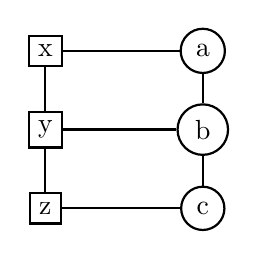
\begin{tikzpicture}\node[shape=rectangle,draw=black,align=center,line width=0.8pt] (0) at (3.0,15.166666666666666) {x};
\node[shape=rectangle,draw=black,align=center,line width=0.8pt] (1) at (3.0,14.166666666666666) {y};
\node[shape=rectangle,draw=black,align=center,line width=0.8pt] (2) at (3.0,13.166666666666666) {z};
\node[shape=circle,draw=black,align=center,line width=0.8pt] (3) at (5.0,15.166666666666666) {a};
\node[shape=circle,draw=black,align=center,line width=0.8pt] (4) at (5.0,14.166666666666666) {b};
\node[shape=circle,draw=black,align=center,line width=0.8pt] (5) at (5.0,13.166666666666666) {c};

\path [-,draw=black,line width=0.8pt] (0) edge node {} (3);
\path [-,draw=black,line width=0.8pt] (1) edge node {} (4);
\path [-,draw=black,line width=0.8pt] (2) edge node {} (5);
\path [-,draw=black,line width=0.8pt] (0) edge node {} (1);
\path [-,draw=black,line width=0.8pt] (1) edge node {} (2);
\path [-,draw=black,line width=0.8pt] (3) edge node {} (4);
\path [-,draw=black,line width=0.8pt] (4) edge node {} (5);
\end{tikzpicture}
\end{document}